%======================================================%
%   Beamer Presentation
%   LaTeX Template
%   compile using PDFTeXify, PDFLaTeX or XeLaTeX
%======================================================%

%--------------------------------------------------------------------------------
%   PACKAGES AND THEMES
%--------------------------------------------------------------------------------

\documentclass[notheorems,10pt,compress]{beamer}

\mode<presentation>{
	
	%------- Beamer theme ------
	\usetheme{Madrid}
	%\usetheme{Boadilla}
	%\usetheme{Frankfurt}
	%\usetheme{Warsaw}
	%\usetheme{CambridgeUS}
	%\usetheme{Montpellier}
	
	%------- Color theme ------
	\usecolortheme{rose}
	%\usecolortheme{orchid}
	%\usecolortheme{lily}
	%\usecolortheme{whale}
	%\usecolortheme{dolphin}
	%\usecolortheme{seahorse}
	
	%\usetheme{boxes}
	%\setbeamercovered{transparent}
	%\usefonttheme[onlymath]{serif}
	\usefonttheme{serif}
	\usefonttheme{professionalfonts}
	
	
	%\setbeamertemplate{headline}{}
	%\setbeamertemplate{footline}{}
	\setbeamertemplate{blocks}[rounded][shadow=true]
	\setbeamertemplate{navigation symbols}{}
	%\setbeamertemplate{itemize items}[square]  % ball, circle, square
	\setbeamertemplate{enumerate items}[default]
	%\setbeamertemplate{section in toc}[square]
	
}

%--------- 宏包  ----------
\usepackage[UTF8,noindent]{ctex}
%\usepackage[english]{babel}
\usepackage{amsmath,amssymb,version}
\usepackage{graphicx,fancybox,mathrsfs,multirow}
\usepackage{booktabs}
\usepackage{epsfig,epstopdf}
\usepackage{url,hyperref}
\usepackage{tabularx,array,makecell}
\usepackage{color,xcolor}
\usepackage{cases}
\usepackage{mathtools}
\usepackage{tikz}
\usepackage{indentfirst}
%---------- 定义行距 ----------
\renewcommand{\baselinestretch}{1.15}

%---------- 定义表格新命令 ----------
\newcolumntype{P}[1]{>{\centering \arraybackslash}p{#1}}
\newcolumntype{L}{>{\quad}X}
\newcolumntype{C}{>{\centering \arraybackslash}X}
\newcolumntype{R}{>{\raggedright \arraybackslash}X}


\newcommand{\RR}{\ensuremath{\mathbb{R}}}
\newcommand{\EE}{\mathbb{E}}

%---------- 设置字体  ----------
\setbeamerfont{normal text}{family=\rmfamily}
\setbeamerfont{frametitle}{family=\rmfamily}
\setbeamerfont{title}{family=\rmfamily}
\setbeamerfont{subtitle}{family=\rmfamily}
\setbeamerfont{institute}{family=\kaishu}
\setbeamerfont{author}{family=\kaishu}
%\setbeamerfont{date}{family=\rmfamily}
\setbeamerfont{footline}{family=\kaishu}
\setbeamerfont{section in toc}{family=\rmfamily}
\setbeamerfont{subsection in toc}{family=\rmfamily}
\AtBeginDocument{\usebeamerfont{normal text}}

\setbeamertemplate{caption}[numbered]
\numberwithin{figure}{section}
\numberwithin{table}{section}
\numberwithin{equation}{section}

%---------- 定理设置  --------------
\setbeamertemplate{theorems}[numbered]
%\newtheorem{theorem}{Theorem}
\newtheorem{theorem}{定理}
\numberwithin{theorem}{section}
%\newtheorem{definition}{Definition}
\newtheorem{definition}{定义}
\numberwithin{definition}{section}
%\newtheorem{lemma}{Lemma}
\newtheorem{lemma}{引理}
\numberwithin{lemma}{section}
%\newtheorem{proposition}{Proposition}
\newtheorem{proposition}{命题}
\numberwithin{proposition}{section}
%\newtheorem{corollary}{Corollary}
\newtheorem{corollary}{推论}
\numberwithin{corollary}{section}
\theoremstyle{example}
%\newtheorem{example}{Example}
\newtheorem{example}{例}
%\numberwithin{example}{section}
\renewenvironment{proof}[1][证明]{\textbf{#1}:~~}{\qed\par}
\newenvironment{solution}{\par\noindent\textbf{解}:~~}{\par}

%---------- 调节公式的间距 ----------
%\AtBeginDocument{
	%	\setlength{\abovedisplayskip}{4pt plus 1pt minus 1pt}
	%	\setlength{\belowdisplayskip}{4pt plus 1pt minus 1pt}
	%	\setlength{\abovedisplayshortskip}{2pt}
	%	\setlength{\belowdisplayshortskip}{2pt}
	%	\setlength{\arraycolsep}{2pt}
	%}


\makeatletter
\newcommand\HUGE{\@setfontsize\Huge{36}{42}}
\makeatother

\def\a{\alpha}
\def\e{\varepsilon} \def\z{\zeta} \def\y{\eta} \def\o{\theta}
\def\vo{\vartheta} \def\k{\kappa} \def\l{\lambda} \def\m{\mu} \def\n{\nu}
%\AtBeginSection[]{
	%\begin{frame}
	%  \frametitle{Outline} %\small
	%  \vskip -5pt
	%  \hspace*{1.5em}
	%  \parbox[t]{.95\textwidth}{
		%  \begin{minipage}[c][0.6\textheight]{\textwidth}
			%  \tableofcontents[currentsection,currentsubsection,subsectionstyle=show/show/shaded]
			%  \end{minipage}
		%  }
	%  \addtocounter{framenumber}{-1}
	%\end{frame}
	%}


%---------- 自定义命令 ----------
\newcommand{\red}[1]{\textcolor{red}{#1}}
\newcommand{\blue}[1]{\textcolor{blue}{#1}}


%--------------------------------------------------------------------------------
%	TITLE PAGE
%--------------------------------------------------------------------------------
\title[加性噪声驱动的时间变换随机微分方程的数值方法]{加性噪声驱动的时间变换随机微分方程的数值方法}

\author[左如春]
{
	答辩人:左如春~~ \vskip 3mm
	% 报告人:学生姓名~~ \vskip 3mm
	专业:计算数学 \vskip 3mm
	指导教师:刘暐 ~ 副研究员 \vskip 3mm
	研究方向:常微分方程数值解
}
%\author[姓名]{报告人姓名}

\institute[上海师范大学]{}
%\institute[学校名称]{\normalsize 学校名称}

\date[2024.09.20]{2024.09.20}


\graphicspath{{./figures/}}

\begin{document}
	
	
	\begin{frame}
		\titlepage
	\end{frame}
	
	\begin{frame}
		\frametitle{Outline}
		\vskip -5.6pt
		\hspace*{1.5em}
		\parbox[t]{.95\textwidth}{
			\begin{minipage}[c][0.6\textheight]{\textwidth}
				\tableofcontents
			\end{minipage}
		}
	\end{frame}
	
	%--------------------------------------------------------------------------------
	%	PRESENTATION SLIDES
	%--------------------------------------------------------------------------------
	\section{研究背景与意义}
	
	\begin{frame}
		\frametitle{1.研究背景与意义}
		
		\begin{itemize}
			\setlength{\itemsep}{10pt}
			\item 时间变换随机过程和时间变换随机微分方程(SDE)作为描述亚扩散过程重要工具之一, 在众多领域发挥着重要作用. 包括: 金融模型、生物化学等领域\footnote{Marcin Magdziarz, Sebastian Orzel, and Aleksander Weron. Option pricing in subdiff-\\
				usive Bachelier model. J.Stat. Phys., 145(1):187–203, 2011.}.
			
			\item 对于时间变换SDE的研究, 目前的数值方法包括Euler型方法、Milstein型方法等. 
		\end{itemize}
		\begin{itemize}
			\setlength{\itemsep}{10pt}
			\item 对于超线性系数的时间变换布朗运动驱动的SDE, 若要获得更高的收敛阶, 
			一般需要采用Milstein方法或其他更高阶的数值方法.
			\item 对于一类可以通过Lamperti变换将漂移项转化为满足单调条件的SDE, 使用BEM方法能够使强收敛阶超过0.5. 
			\item 时间变换的SDE的真实解解很少能显式地表达出来, 因此其数值逼近尤为重要.
		\end{itemize}
	\end{frame}
	
%	\begin{frame}		
%		\frametitle{\zihao{-4} 1.2 研究意义}
%		
%		\begin{itemize}
%			\setlength{\itemsep}{10pt}
%			\item 具有超线性系数的时间变换布朗运动驱动的SDE,要想得到更高的强收敛阶, 一般只能采用Milstein或其它更高阶的数值方法.
%			\item 对于一类能够通过Lamperti变换成漂移项满足单调条件的SDE, 通过BEM可以使强收敛阶超过0.5.
%			\item 时间变换的SDE的真实解解很少能显式地表达出来, 因此其数值逼近尤为重要.
%			
%			
%		\end{itemize}
%	\end{frame}
	
	
	\section{国内外研究现状}
	
	\begin{frame}
		\frametitle{2.国内外研究现状}
		\begin{itemize}
			\setlength{\itemsep}{10pt}
			\item \blue{ Alfonsi(2013) } 单调条件, Lamperti变换, BEM, 强收敛. 
			\item \blue{Neuenkirch, Szpruch(2014)} 单边Lipschitz, Lamperti变换, BEM, 强收敛.
			\item \blue{ Yang, Huang(2021) } SIS模型, Lamperti变换, 对数EM, 强收敛.
		\end{itemize}
		\begin{itemize}
			\setlength{\itemsep}{10pt}
			\item \blue{ Jum, Kobayashi(2016) } 全局Lipschitz, 对偶原则, EM, 强弱收敛.
			\item \blue{ Jin, Kobayashi(2019) }  全局Lipschitz, H\"{o}lder连续, 非等距EM, 强收敛
			\item \blue{ Deng, Liu(2020) } 单边Lipschitz, H\"{o}lder连续, 半隐式EM, 强收敛, 均方稳定. 
			\item \blue{Liu, Mao, Tang, Wu(2020) } 单边Lipschitz,  H\"{o}lder连续, 对偶原则, 截断EM, 强收敛.
		\end{itemize}
	\end{frame}
	
	%------------------------------------------------
	\section{研究内容与主要工作}
	%------------------------------------------------
	
	\begin{frame}
		\frametitle{3.研究内容与主要工作\\\zihao{-4} 3.1 研究内容}
%		\setlength{\parindent}{2em}下面是一种具有稳定指数为$\alpha$的特殊L\'{e}vy过程D, 及其逆从属E的示意图:
		\begin{figure}[!htp]
			\begin{minipage}[h]{0.48\linewidth}
				\centering
				\includegraphics[width=0.9\linewidth]{D的概念图.eps}
				\caption{具有稳定指数$\alpha$的从属D}
				\label{CIRrate}
			\end{minipage}
			\begin{minipage}[h]{0.48\linewidth}
				\centering
				\includegraphics[width=0.9\linewidth]{E的概念图.eps}%width=\textwidth
				\caption{逆从属E}
				\label{CEVrate}
			\end{minipage}
		\end{figure}
	\end{frame}
	
	\begin{frame}		
		\frametitle{\zihao{-4} 3.1 研究内容}
	    \setlength{\parindent}{2em}对于下面的时间变换SDE:
	    \begin{equation*}
	    	dy(t)=a(y(t))dE(t)+b(y(t))dB(E(t)),~t\geq0,~y(0)\in S.
	    \end{equation*}
	    通过Lamperti变换
	    \begin{equation*}\label{Lamperti}
	    	F(x)=\lambda\int^x\frac1{b(y)}dy.
	    \end{equation*}
	    将乘性噪声转变成加性噪声
    	\begin{equation*}\label{SDE}
    		dx(t)=f(x(t))dE(t) + \lambda dB(E(t)), ~ t\geq0,~x(0)\in F(S).
    	\end{equation*}
	    
	    其中
	    \begin{equation*}
	    	f(x)=\lambda\left(\frac{a(F^{-1}(x))}{b(F^{-1}(x))}-\frac12b^{\prime}(F^{-1}(x))\right),~ x\in F(S).
	    \end{equation*}
	    这里$t\in S=(l,r)$, 其中 $-\infty\leq l<r\leq\infty$.
	    对所有 $q > 0$有$\EE |x_0|^q < \infty$.  函数 $a,b$是$S\to S$ 的连续可微函数.
		
	\end{frame}
	
	\begin{frame}		
		\frametitle{\zihao{-4} 3.2 主要工作}
		%\begin{block}{}
		\hspace{2em}经过Lamperti变换后的时间变换SDE, 漂移项系数$f$满足以下条件:
		\begin{itemize}
			\setlength{\itemsep}{0.1pt}
			\item  $f$满足单调条件
			\begin{equation}
				f:~I\to\mathbb{R}  ,~使得 \exists K \in\mathbb{R},~\forall x,~y\in I,~x\leq y,~f(y)-f(x)\leq K(y-x).
			\end{equation}  
			\item $f$是二阶连续可微的并且满足
			\begin{equation}
				\sup\limits_{t\in[0,T]}\mathbb{E}\left|f'(x(t))\right|+
				\sup\limits_{t\in[0,T]}\mathbb{E}\left|f'(x(t))f(x(t))+
				\frac{\sigma^2}2f''(x(t))\right|<\infty.
			\end{equation}
		\end{itemize}
		\hspace{2em}在此基础之上, 我们研究一类时间变换SDE的BEM方法的强收敛阶.

	\end{frame}
	
	\begin{frame}		
		\frametitle{\zihao{-4} 3.2 主要工作}
		\setlength{\parindent}{2em}具体工作如下:
		\vskip 5pt
		\begin{itemize}
			\setlength{\itemsep}{5pt}
			\item 建立逆从属$E(t)$在$\Delta t$时间内的期望$\mathbb{E}\left[\Delta E(t)\right]^n$与$\Delta t$之间的关系.
			\begin{equation*}
				\mathbb{E}[\Delta E(t)]^n \le C\Delta t^{1+(n-1)\alpha}
			\end{equation*}
			\item 证明真实解和数值解的矩有界.
			\item 结合It\^{o}公式、Cauchy-Schwarz不等式、BDG不等式和Gronwall’s不等式等证明BEM数值方法的强收敛, 并给出强收敛阶.
			\begin{equation*}
					\mathbb{E}\left[\sup_{0\leq t\leq T}|x({t_i})-x_{t_i}|\right]\le C\Delta t^\alpha
			\end{equation*}
			\item 给出时间变换SDE的BEM方法的实现代码, 通过时间变换CIR和CEV过程的数值算例对理论结果进行验.
		\end{itemize}
	\end{frame}
	
%	\begin{frame}		
%		\frametitle{\zihao{-4} 3.2 主要工作}
%		\setlength{\parindent}{2em}本论文通过两个数值算例进行理论验证:
%		\vskip 5pt
%		\begin{itemize}
%			\setlength{\itemsep}{5pt}
%			\item 考虑由时间变换布朗运动驱动的CIR过程:
%			\begin{equation*}
%					dy(t)=(\frac14-2y(t))dE(t)+\frac12\sqrt{y(t)}dB(E(t)).
%			\end{equation*}
%		Lamperti变换之后
%		\begin{equation}
%			dX(t)=\left(\frac{3}{32}X(t)^{-1} - X(t)\right)dE(t)+\frac14dB(E(t))
%		\end{equation}
%			\item 考虑由时间变换布朗运动驱动的CEV过程:
%			\begin{equation*}
%					dy(t)=(1-y(t))dE(t)+ y(t)^{\frac45} dB(E(t))
%			\end{equation*}
%			Lamperti变换之后
%			\begin{equation}
%				dX(t)=\left(\frac15 X(t)^{-4} - \frac15 X(t) - \frac{2}{25} X(t)^{-1}\right)dE(t)+\frac15 dB(E(t))
%			\end{equation}
%		
%		\end{itemize}
%	\end{frame}
	
	
%	\begin{frame}		
%		\frametitle{\zihao{-4} 3.2 主要工作}
%		由稳定指数为$\alpha$的D驱动的时间变换CIR和CEV过程的BEM方法数值结果:
%		
%		\begin{figure}[!htp]
%			\begin{minipage}[h]{0.48\linewidth}
%				\centering
%				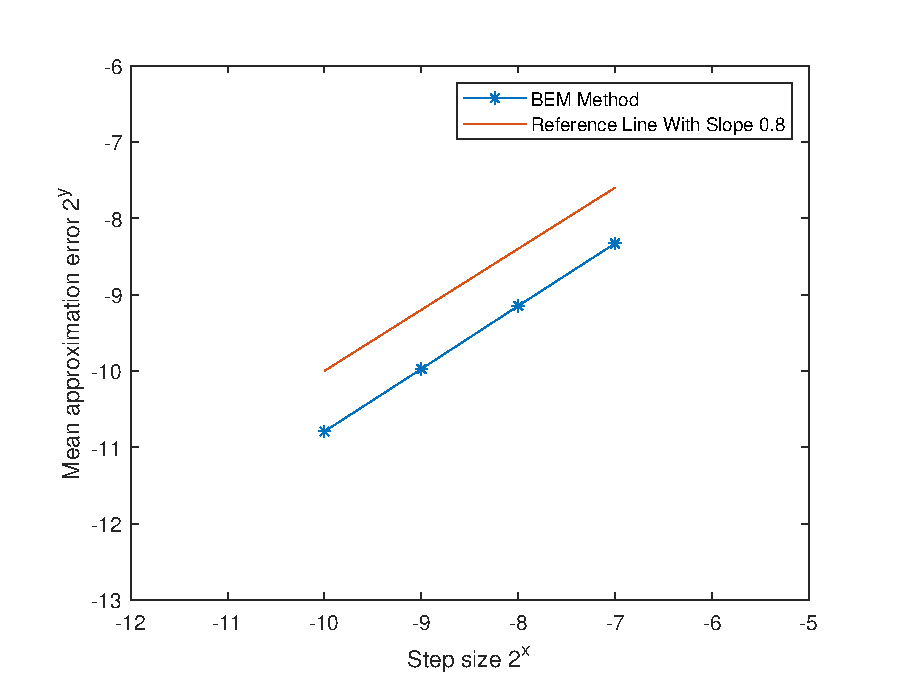
\includegraphics[width=0.9\linewidth]{BEMalpha=0.8.eps}
%				\caption{0.8-稳定驱动的CIR过程}
%				\label{CIRrate}
%			\end{minipage}
%			\begin{minipage}[h]{0.48\linewidth}
%				\centering
%				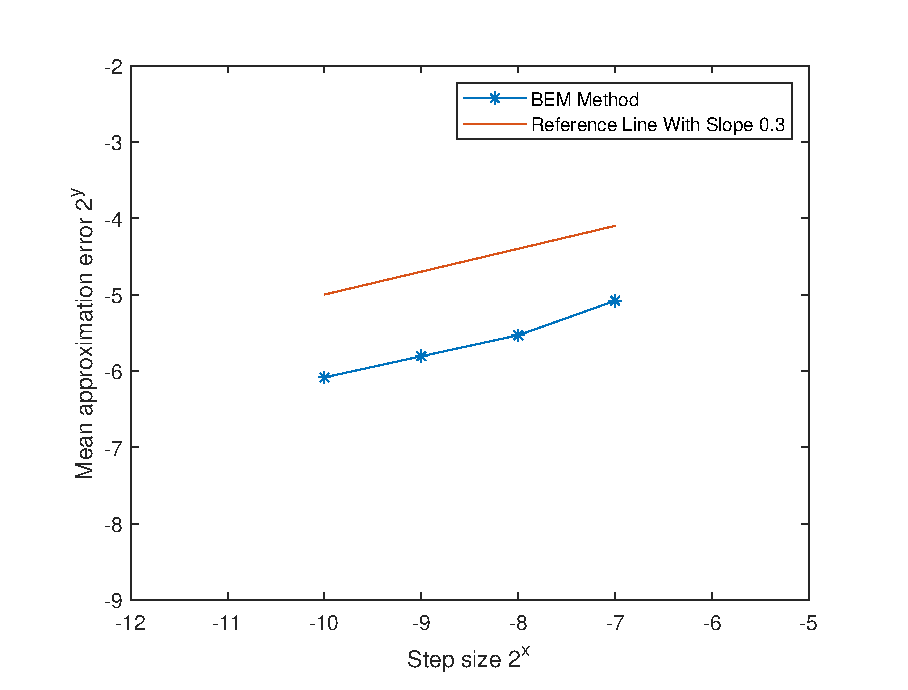
\includegraphics[width=0.9\linewidth]{BEMalpha=0.3.eps}%width=\textwidth
%				\caption{CEV过程强收敛率为0.3}
%				\label{CEVrate}
%			\end{minipage}
%		\end{figure}
%	\end{frame}
	%------------------------------------------------
	\section{论文创新点与问题}
	
	
	\begin{frame}{论文创新点与问题}
		\frametitle{4.论文创新点与问题}
		\begin{block}{}
			\vskip 6pt
			\begin{itemize}
				\setlength{\itemsep}{6pt}
				\item 本文通过引入Lamperti变换,将时间变换SDE的乘性噪声转化成加性噪声,方便处理噪声项.
				\item 在数值方法中,我们考虑对$t$直接等距离散,从而得到收敛阶与$\alpha$的关系.
				\item 由于引入的是对时间$t$的等距离散,导致取期望时微分项$dE(t)$不能直接放缩,因此很多经典SDE和时间变换SDE的结果都无法直接使用.
				\item 当从属$D$的稳定指数$\alpha < 0.5$时, 收敛阶与预期结果之间相差较大.
			\end{itemize}
		\end{block}
	\end{frame}
	
	\section{论文进度安排}
	
	
	
	\begin{frame}{论文进度安排}
		\frametitle{5.论文进度安排}
		\begin{table}[htp!]
			\centering
			\renewcommand\arraystretch{1.5} %定义表格高度
			% PLCR前面已经定义
			\begin{tabularx}{0.8\textwidth}{|P{2.8cm}|C|}
				\Xhline{2\arrayrulewidth}
				\textbf{起止时间}       &  \textbf{论文进度安排}\\
				\hline
				2024.02 - 2024.03    &  论文定题, 收集、阅读并整理相关文献\\
				\hline
				2024.04 - 2024.07    &  完成$E(t)$在等距区间的估计,并整理\\
				\hline
				2024.08 - 2024.09    &  论文撰写、修改、完成开题报告\\
				\hline
				2024.10 - 2024.11    & 推导过程和数值模拟总结\\
				\hline
				2024.12 - 2025.01    &  毕业论文预答辩\\
				\hline
				2025.02 - 2025.04    &  补充、完善论文, 论文定稿\\
				\hline
				2025.05    &  毕业论文答辩\\
				\Xhline{2\arrayrulewidth}
			\end{tabularx}
		\end{table}
		
	\end{frame}
	
%	\begin{frame}
%		\frametitle{\zihao{-4} 5.2 预期成果}
%		\begin{block}{}
%			\hspace{2em}本论文研究一类由Lamperti变换成漂移项满足单调条件的SDE的BEM方法, 其\alert{预期成果}如下:
%			\vskip 6pt
%			\begin{itemize}
%				\setlength{\itemsep}{6pt}
%				\item 建立逆从属$E(t)$的期望$\mathbb{E}\left[\Delta E(t)^n\right]$与$\Delta t$之间的关系.
%				\item 验证BEM数值方法的强收敛性, 并给出强收敛率.
%				\item 给出时间变换SDE的BEM方法的实现代码, 通过时间变换CIR和CEV过程数值算例对理论结果进行验证, 形成研究论文.
%			\end{itemize}
%		\end{block}
%	\end{frame}
	
	%-----------------------------------------------
%	\section{主要参考文献}
%	
%	
%	\begin{frame}
%		\frametitle{6.主要参考文献\\\zihao{-4}}
%		
%		
%		\textcolor[rgb]{0.00,0.00,1.00}{对Lamperti变换SDE的研究:}
%		\begin{itemize}
%			
%			\item  Alfonsi A. Strong order one convergence of a drift implicit euler scheme: Application to the cir process[J]. Statistics and Probability Letters, 2013, 83(2):602–607.
%			\item Neuenkirch A,Szpruch L.First order strong approximations of scalar sdes defined in a domain[J].Numerische Mathematik,2014,128:103-136.
%			\item Chen L,Gan S,Wang X.First order strong convergence of an explicit scheme for the stochastic sis epidemic model[J].Journal of Computational and Applied Mathematics,2021,392:113482.
%			
%			
%		\end{itemize}
%	\end{frame}
	
	
%	\begin{frame}
%		\frametitle{6.主要参考文献\\\zihao{-4}}
%		\textcolor[rgb]{0.00,0.00,1.00}{对时间变换SDE数值方法的研究:}
%		\begin{itemize}
%			\item Ernest Jum and Kei Kobayashi. A strong and weak approximation scheme for stochastic differential equations driven by a time-changed Brownian motion. Probab. Math. Statist., 36(2):201–220, 2016.
%			\item Sixian Jin and Kei Kobayashi. Strong approximation of time-changed stochastic differential equations involving drifts with random and non-random integrators. BIT, 61(3):829–857, 2021.
%			\item Magdziarz M. Stochastic representation of subdiffusion processes with time-dependent drift[J].Stochastic Processes and their Applications, 2009, 119(10):3238-3252.
%			
%		\end{itemize}
%	\end{frame}
	
	
	
	\begin{frame}{}
	    \addtocounter{framenumber}{-1}
		\vskip 1cm
		\begin{center}
			\sffamily
			\HUGE{\textcolor[RGB]{1,8,9}{\zihao{-1}请各位老师批评指正!\\[1mm]谢谢!}}
			%\includegraphics[width=\textwidth]{Thankyou2}
		\end{center}
	\end{frame}
	
	%------------------------------------------------
	
\end{document}
